\section{E. 지도 설치}

\begin{frame} % No title at first slide
    \sectiontitle{E}{지도 설치}
    \sectionmeta{
        \texttt{network\_flow}\\
        출제진 의도 -- \textbf{\color{acdiamond}Challenging}
    }
    \begin{itemize}
        \item 제출 28번, 정답 3팀 (정답률 10.71\%)
        \item 처음 푼 팀: \textbf{정우팬클럽} (회장, 부회장, 정우), 199분
        \item 출제자: \texttt{Diuven}
    \end{itemize}
\end{frame}

\begin{frame}{\textbf{E}. 지도 설치}

    \begin{itemize}
        \item 단순 방향 그래프 $G = (V, E)$, 두 정점 $S, E$, 각 정점별 비용 $C_v$, 자연수 $K \leq 5$
        \item 비용의 합이 최소이면서 다음의 조건을 만족하는 정점 집합 $X$를 찾는 것이 목표입니다.
        \item 조건: $S$에서 $E$로 가는 모든 경로들이 $X$의 원소를 적어도 $K$개 포함하는 것
    \end{itemize}
    
    \begin{center}
        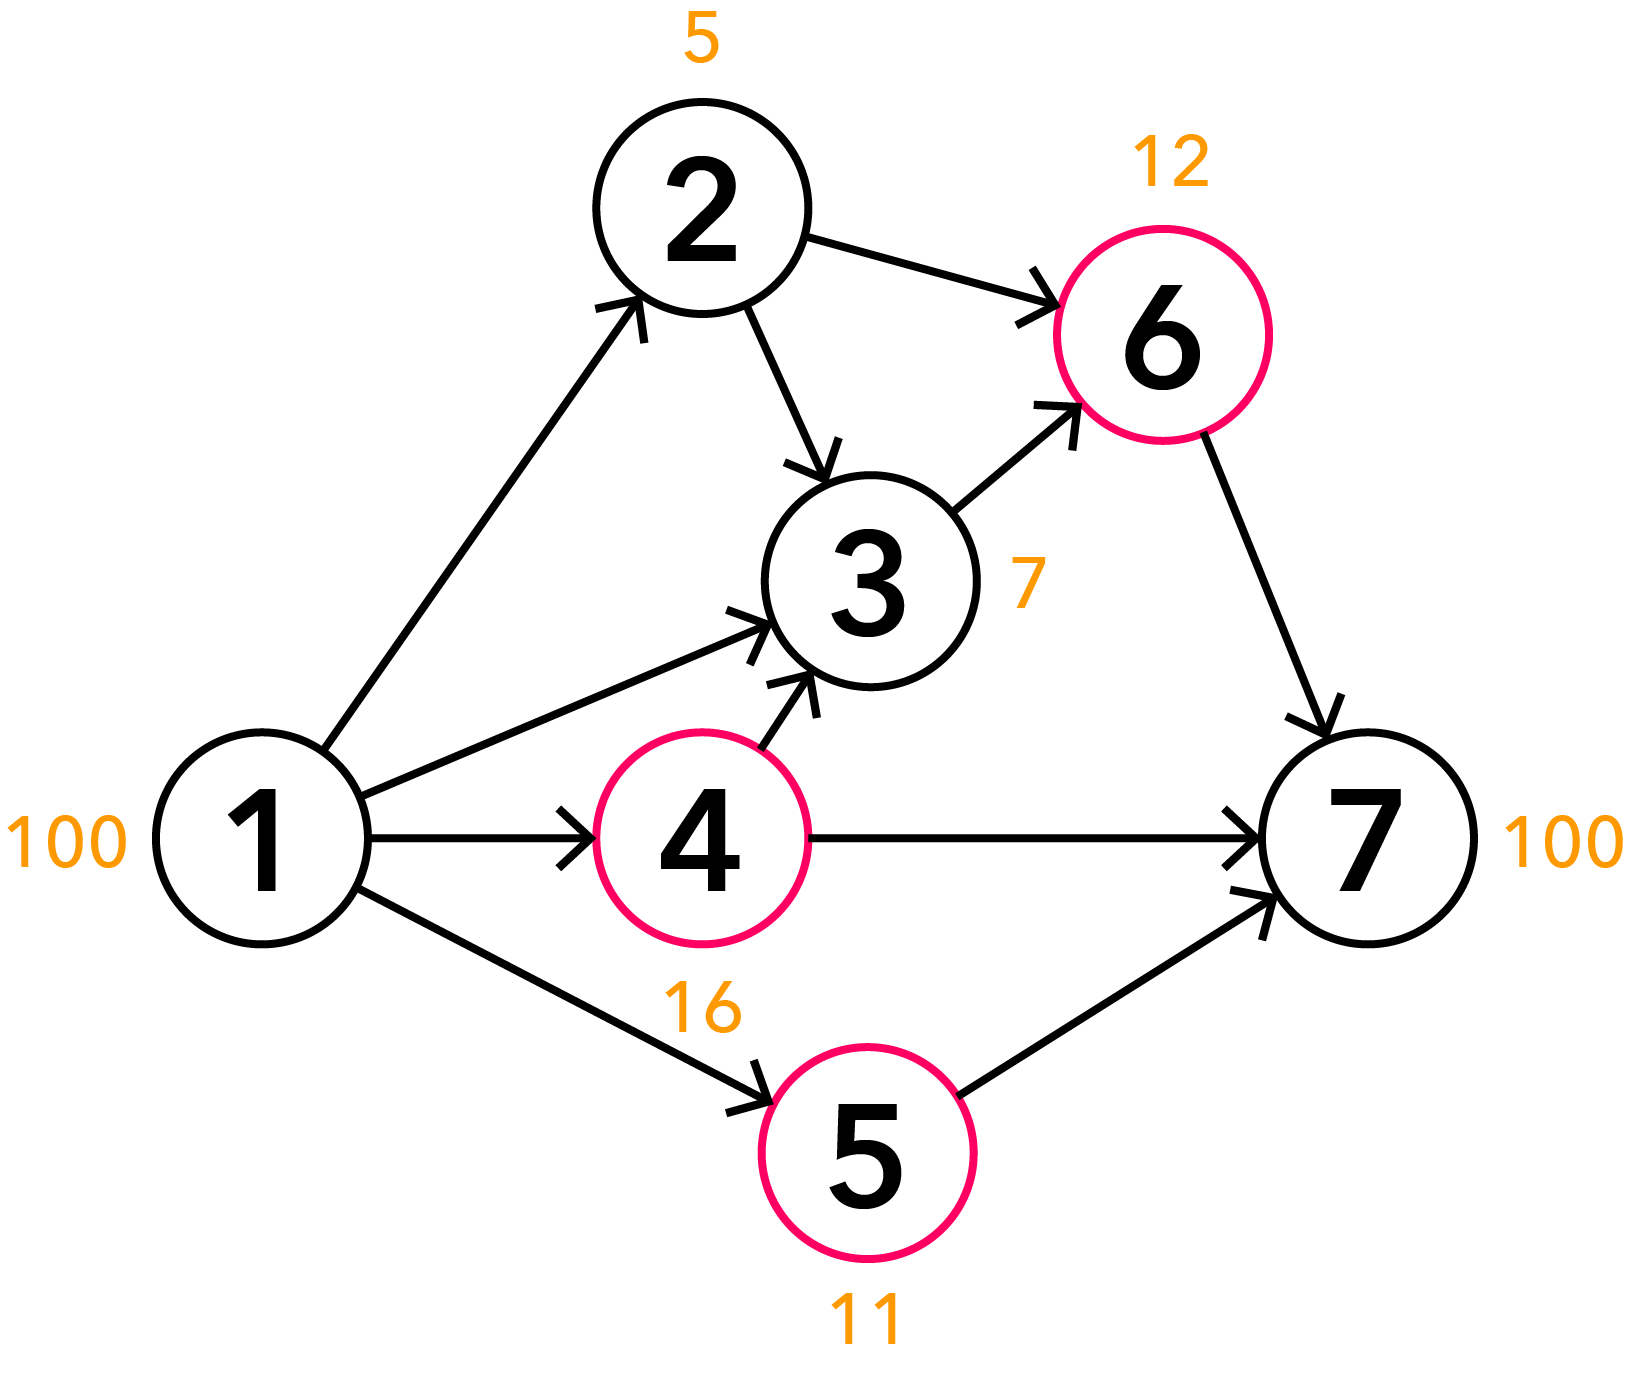
\includegraphics[width=0.3\linewidth]{../images/setting-maps/maps_ex_1.png}
    \end{center}
    
\end{frame}


\begin{frame}{\textbf{E}. 지도 설치}

    $K = 1$인 경우를 풀어봅시다.
    \begin{itemize}
        \item 정점 집합 $X$로 그래프 $G$를 '쪼개면' 됩니다.
        \item 네트워크 플로우 알고리즘으로 s-t edge min cut을 구할 수 있습니다.
        \item 모든 정점을 $v_{in}, v_{out}$ 두 개로 나누고, 들어오는 간선과 나가는 간선을 따로 담당합니다.
        \item $v_{in} \rightarrow v_{out}$ 간선을 추가하고, capacity를 $C_v$로 정합니다.
        \item 나머지 간선들은 모두 capacity를 $\infty$로 설정합니다. (이론상 최대 유량보다 큰 값)
    \end{itemize}
    
    이 그래프에서 $S - E$ max flow를 구하면, 가능한 최소 비용을 구할 수 있습니다.
    
    \vspace{0.5 \baselineskip}
    
    편의상 $v_{in} \rightarrow v_{out}$인 간선들을 Type V 간선, 나머지 간선들을 Type E 간선이라고 부릅시다.

\end{frame}


\begin{frame}{\textbf{E}. 지도 설치}

    \begin{center}
        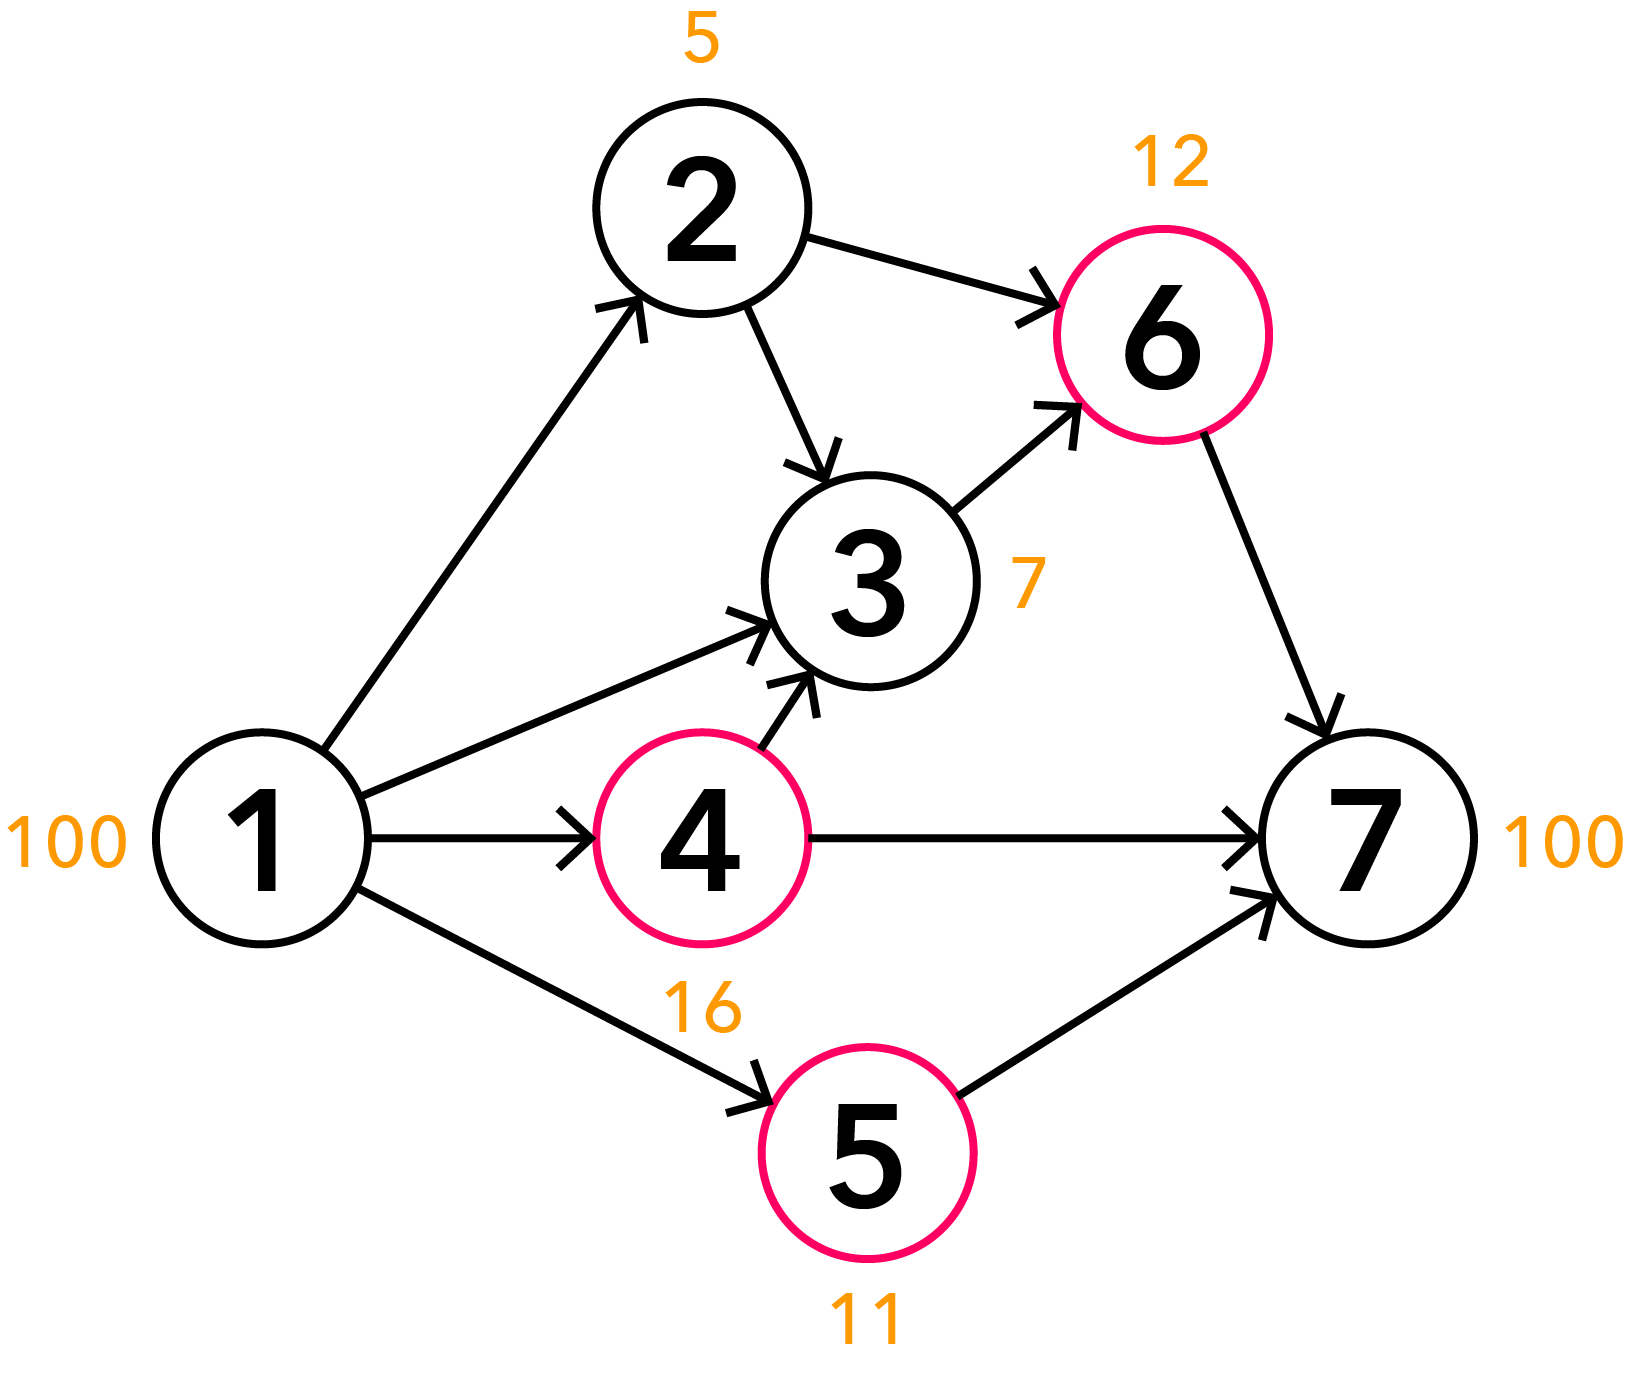
\includegraphics[width=0.45\linewidth]{../images/setting-maps/maps_ex_1.png}
        \hspace{0.05\linewidth}
        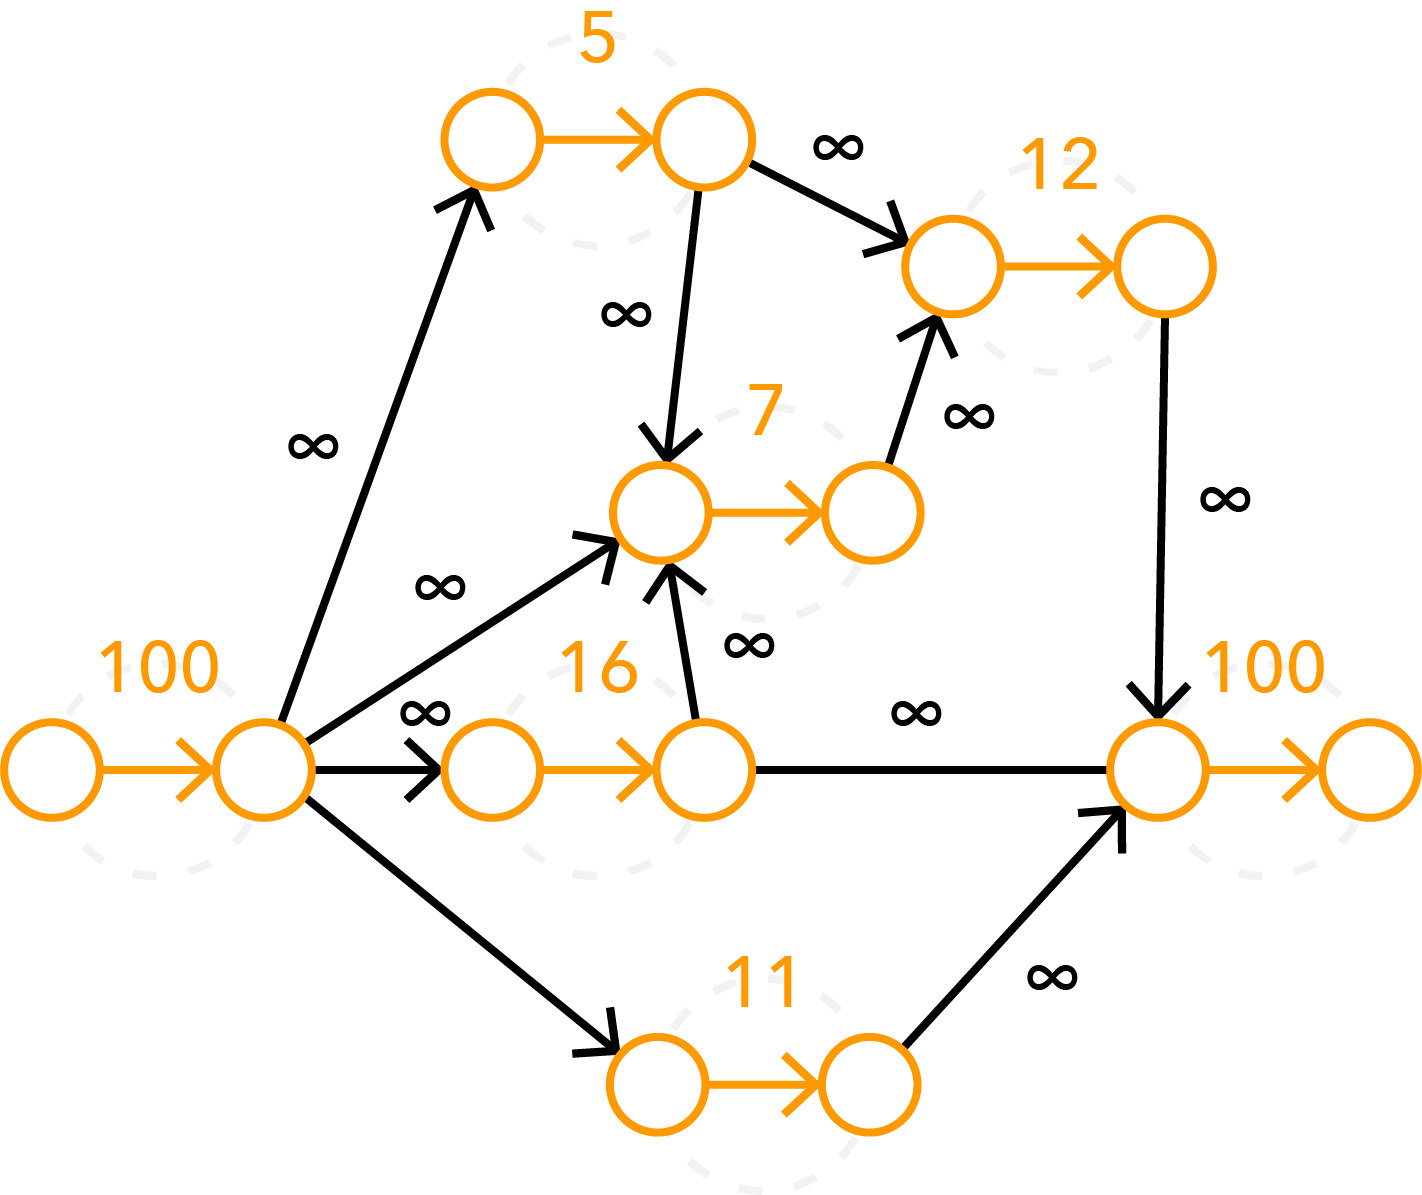
\includegraphics[width=0.45\linewidth]{../images/setting-maps/maps_sol_1.png}
    \end{center}

\end{frame}


\begin{frame}{\textbf{E}. 지도 설치}

    $K > 1$인 경우
    \begin{enumerate}
        \item $K=1$인 경우의 플로우 그래프를 $K$개 만듭니다. \newline
            $z$번째 플로우 그래프를 $G_z$이라고 하고, $G_z$에 속하는 정점들을 ${^z v}$처럼 부릅시다.
        \item 모든 정점에 대해서, $^z v _{in}$과 $^{z+1} v_{out}$를 가중치가 무한대인 간선으로 잇습니다. (Type Z 간선)
        \item super-source와 super-sink에 사용할 두 정점 $A$와 $B$를 만듭니다.
        \item 모든 $z$에 대해 $A \rightarrow {^z S_{in}}$, ${^z E_{out}} \rightarrow B$를 가중치가 무한대인 간선으로 잇습니다. (Type S 간선)
    \end{enumerate}
    
    다음의 그림처럼, 동일한 그래프를 $K$개 만들어 쌓았다고 생각하고, Type Z 간선들이 그 그래프를 z축으로 연결한다고 생각합시다.
    
\end{frame}


\begin{frame}{\textbf{E}. 지도 설치}

    \begin{center}
        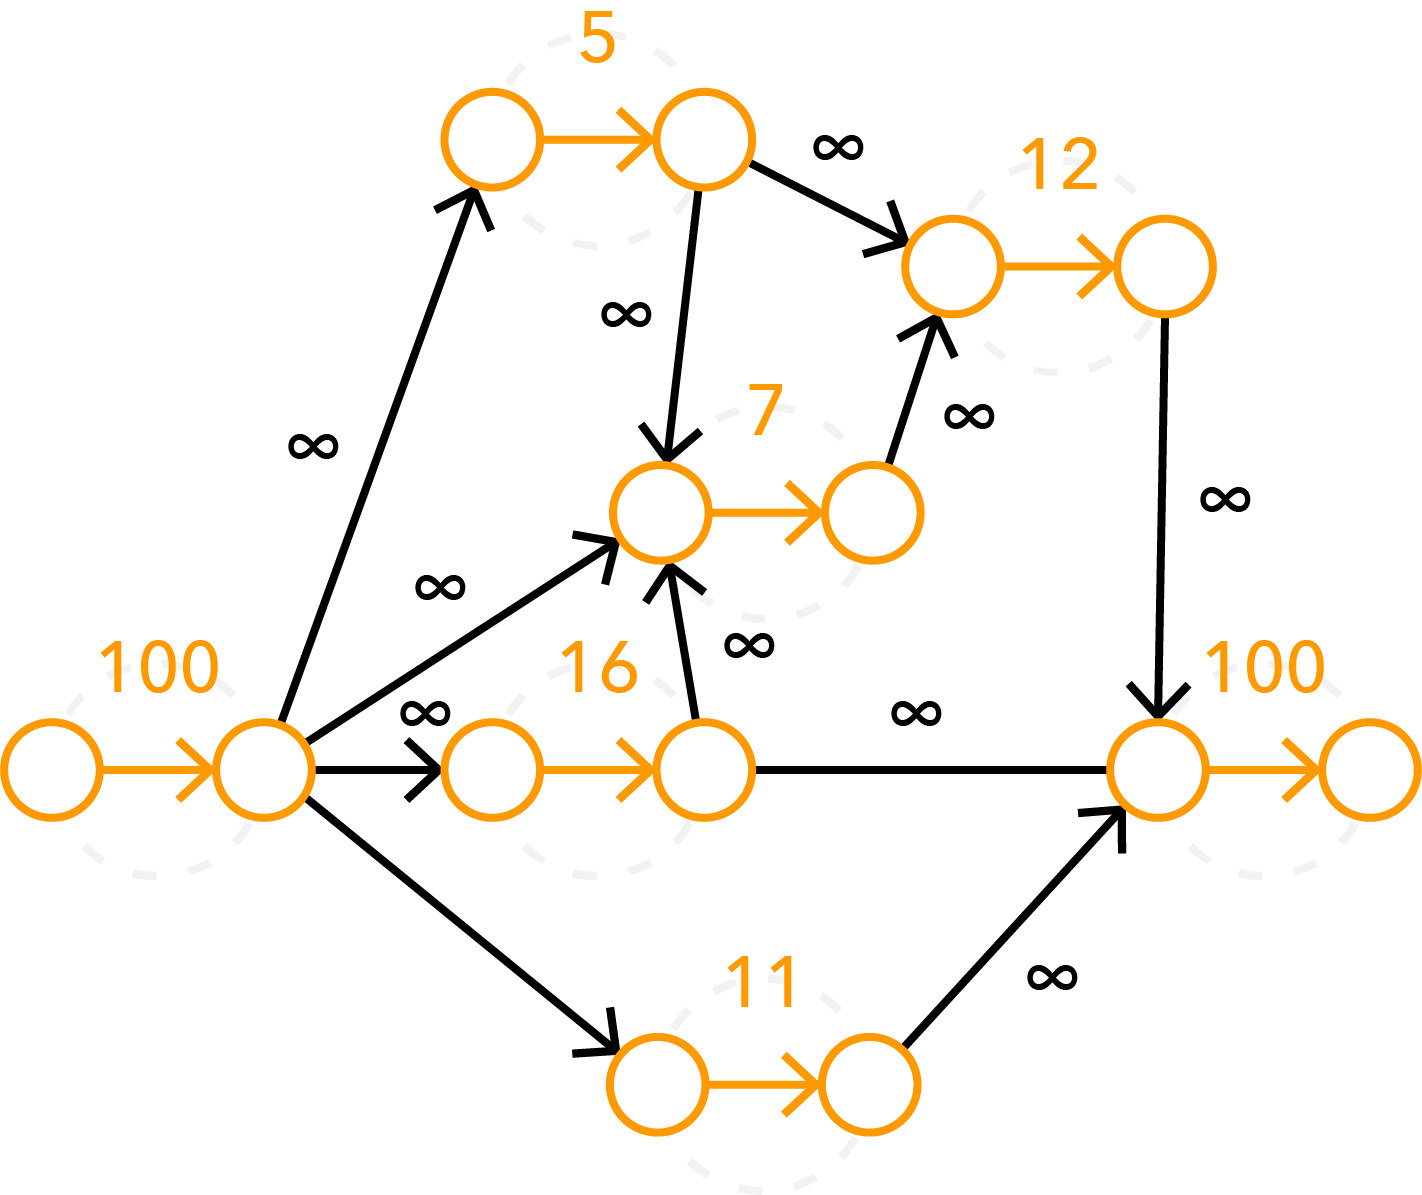
\includegraphics[width=0.45\linewidth]{../images/setting-maps/maps_sol_1.png}
        \hspace{0.05\linewidth}
        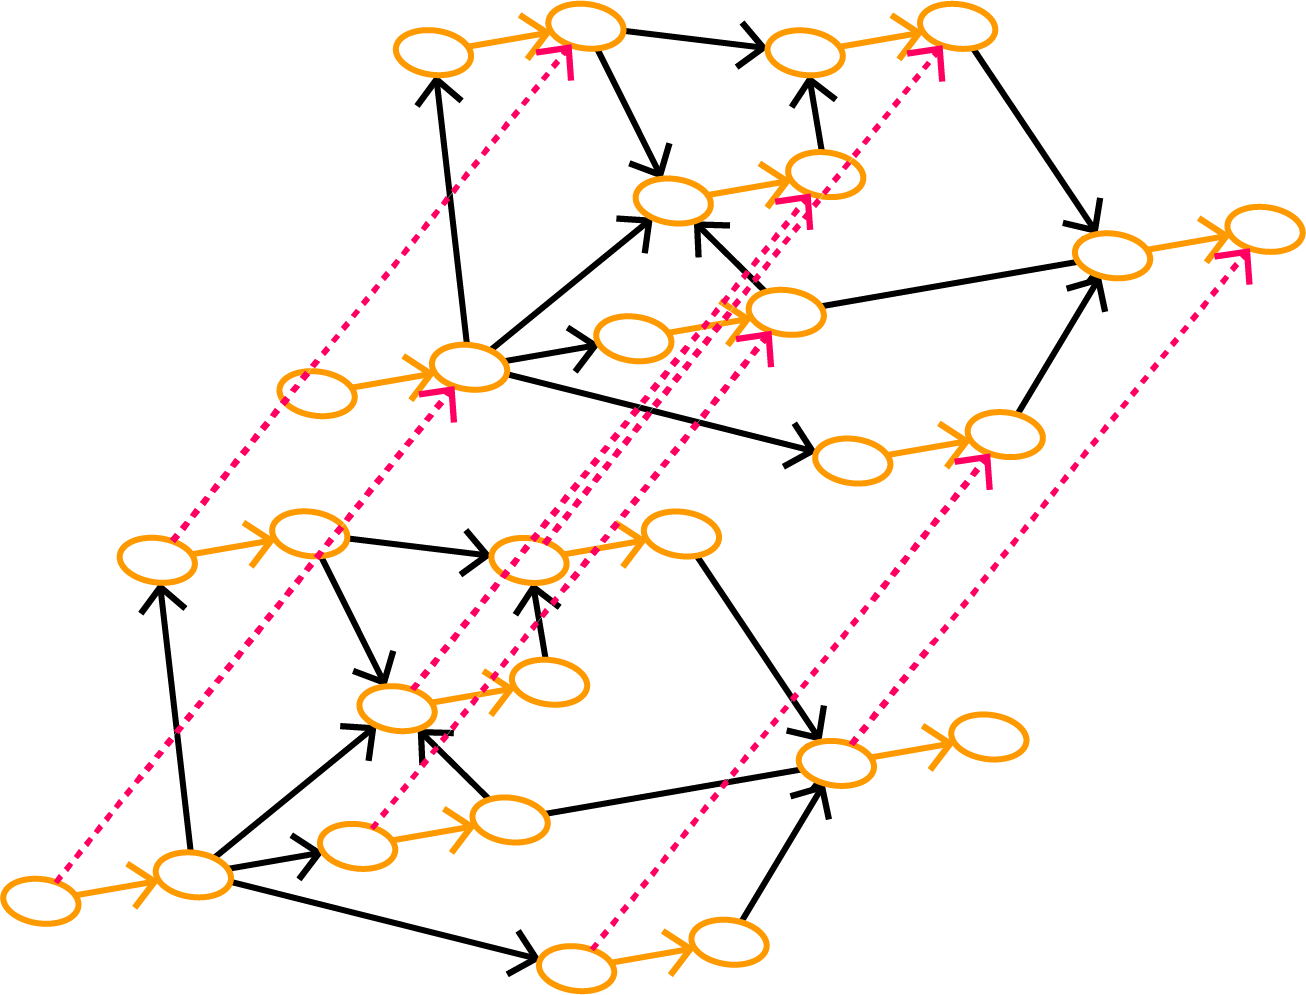
\includegraphics[width=0.45\linewidth]{../images/setting-maps/maps_sol_2.png}
    \end{center}
    
    그림에는 정점 $A, B$와 Type S 간선들이 생략되어 있습니다.

\end{frame}


\begin{frame}{\textbf{E}. 지도 설치}

    이 그래프에서 $K=1$일 때처럼 $A - B$ max flow를 구하면 가능한 최소 비용을 구할 수 있습니다.
    
    \begin{itemize}
        \item 경로를 지나가면서, 지도를 무시하고 지나갈 수 있는 '찬스'가 $K-1$개 있다고 합시다.
        \item 플로우를 구할 때 Type Z 간선을 사용한다는 것은 찬스를 사용하는 것을 의미합니다. \newline
              즉, Type V 간선이 막혀 있을 때 Type Z 간선을 통해 한 층 위로 올라갈 수 있는 것입니다.
        \item 그래프에 max flow를 흘려 주었을 때, $A$에서 $B$로 가는 경로들은 전부 플로우로 막혀 있습니다.
        \item 막힌 간선은 모두 Type V 간선입니다. 따라서 $A$에서 지도를 $K$번 미만 거쳐서 $B$로 갈 수 없습니다.
    \end{itemize}
    
    
\end{frame}


\begin{frame}{\textbf{E}. 지도 설치}

    일반적인 플로우 그래프에서 max flow를 흘려 주었을 때 min cut을 구하는 방법:
    \begin{enumerate}
        \item 플로우 그래프에서 '뚫린 간선'을 잔여 용량이 0이 아닌 간선들이라고 합시다.
        \item (super) source 정점에서 '뚫린 간선'들만 사용해서 도달 가능한 정점들을 체크합니다.
        \item 어떤 간선의 한쪽 끝점은 도달가능하고 다른 한쪽은 불가능한 경우 그 간선은 cut에 속하게 됩니다.
    \end{enumerate}
    
    \vspace{0.5 \baselineskip}
    
    cut에 속하는 간선들은 모두 Type V 간선들이고, 그 간선에 해당하는 정점들이 우리가 구하고자 하는 정점 집합 $X$를 이룹니다.
    
\end{frame}


\begin{frame}{\textbf{E}. 지도 설치}

    min cut을 구하고 cut 정점들의 $C_v$를 무한대로 만드는 과정을 $K$번 반복하는 풀이는 틀립니다.
    
    한 min cut이 한 경로를 여러 번 막는 경우에 답을 구하지 못합니다.
    
    \vspace{0.5 \baselineskip}
    
    아래와 같은 경우, 최적해가 아닌 ${2, 3, 4, 5, 6, 7, 8}$를 선택하게 됩니다.
    
    \begin{center}
        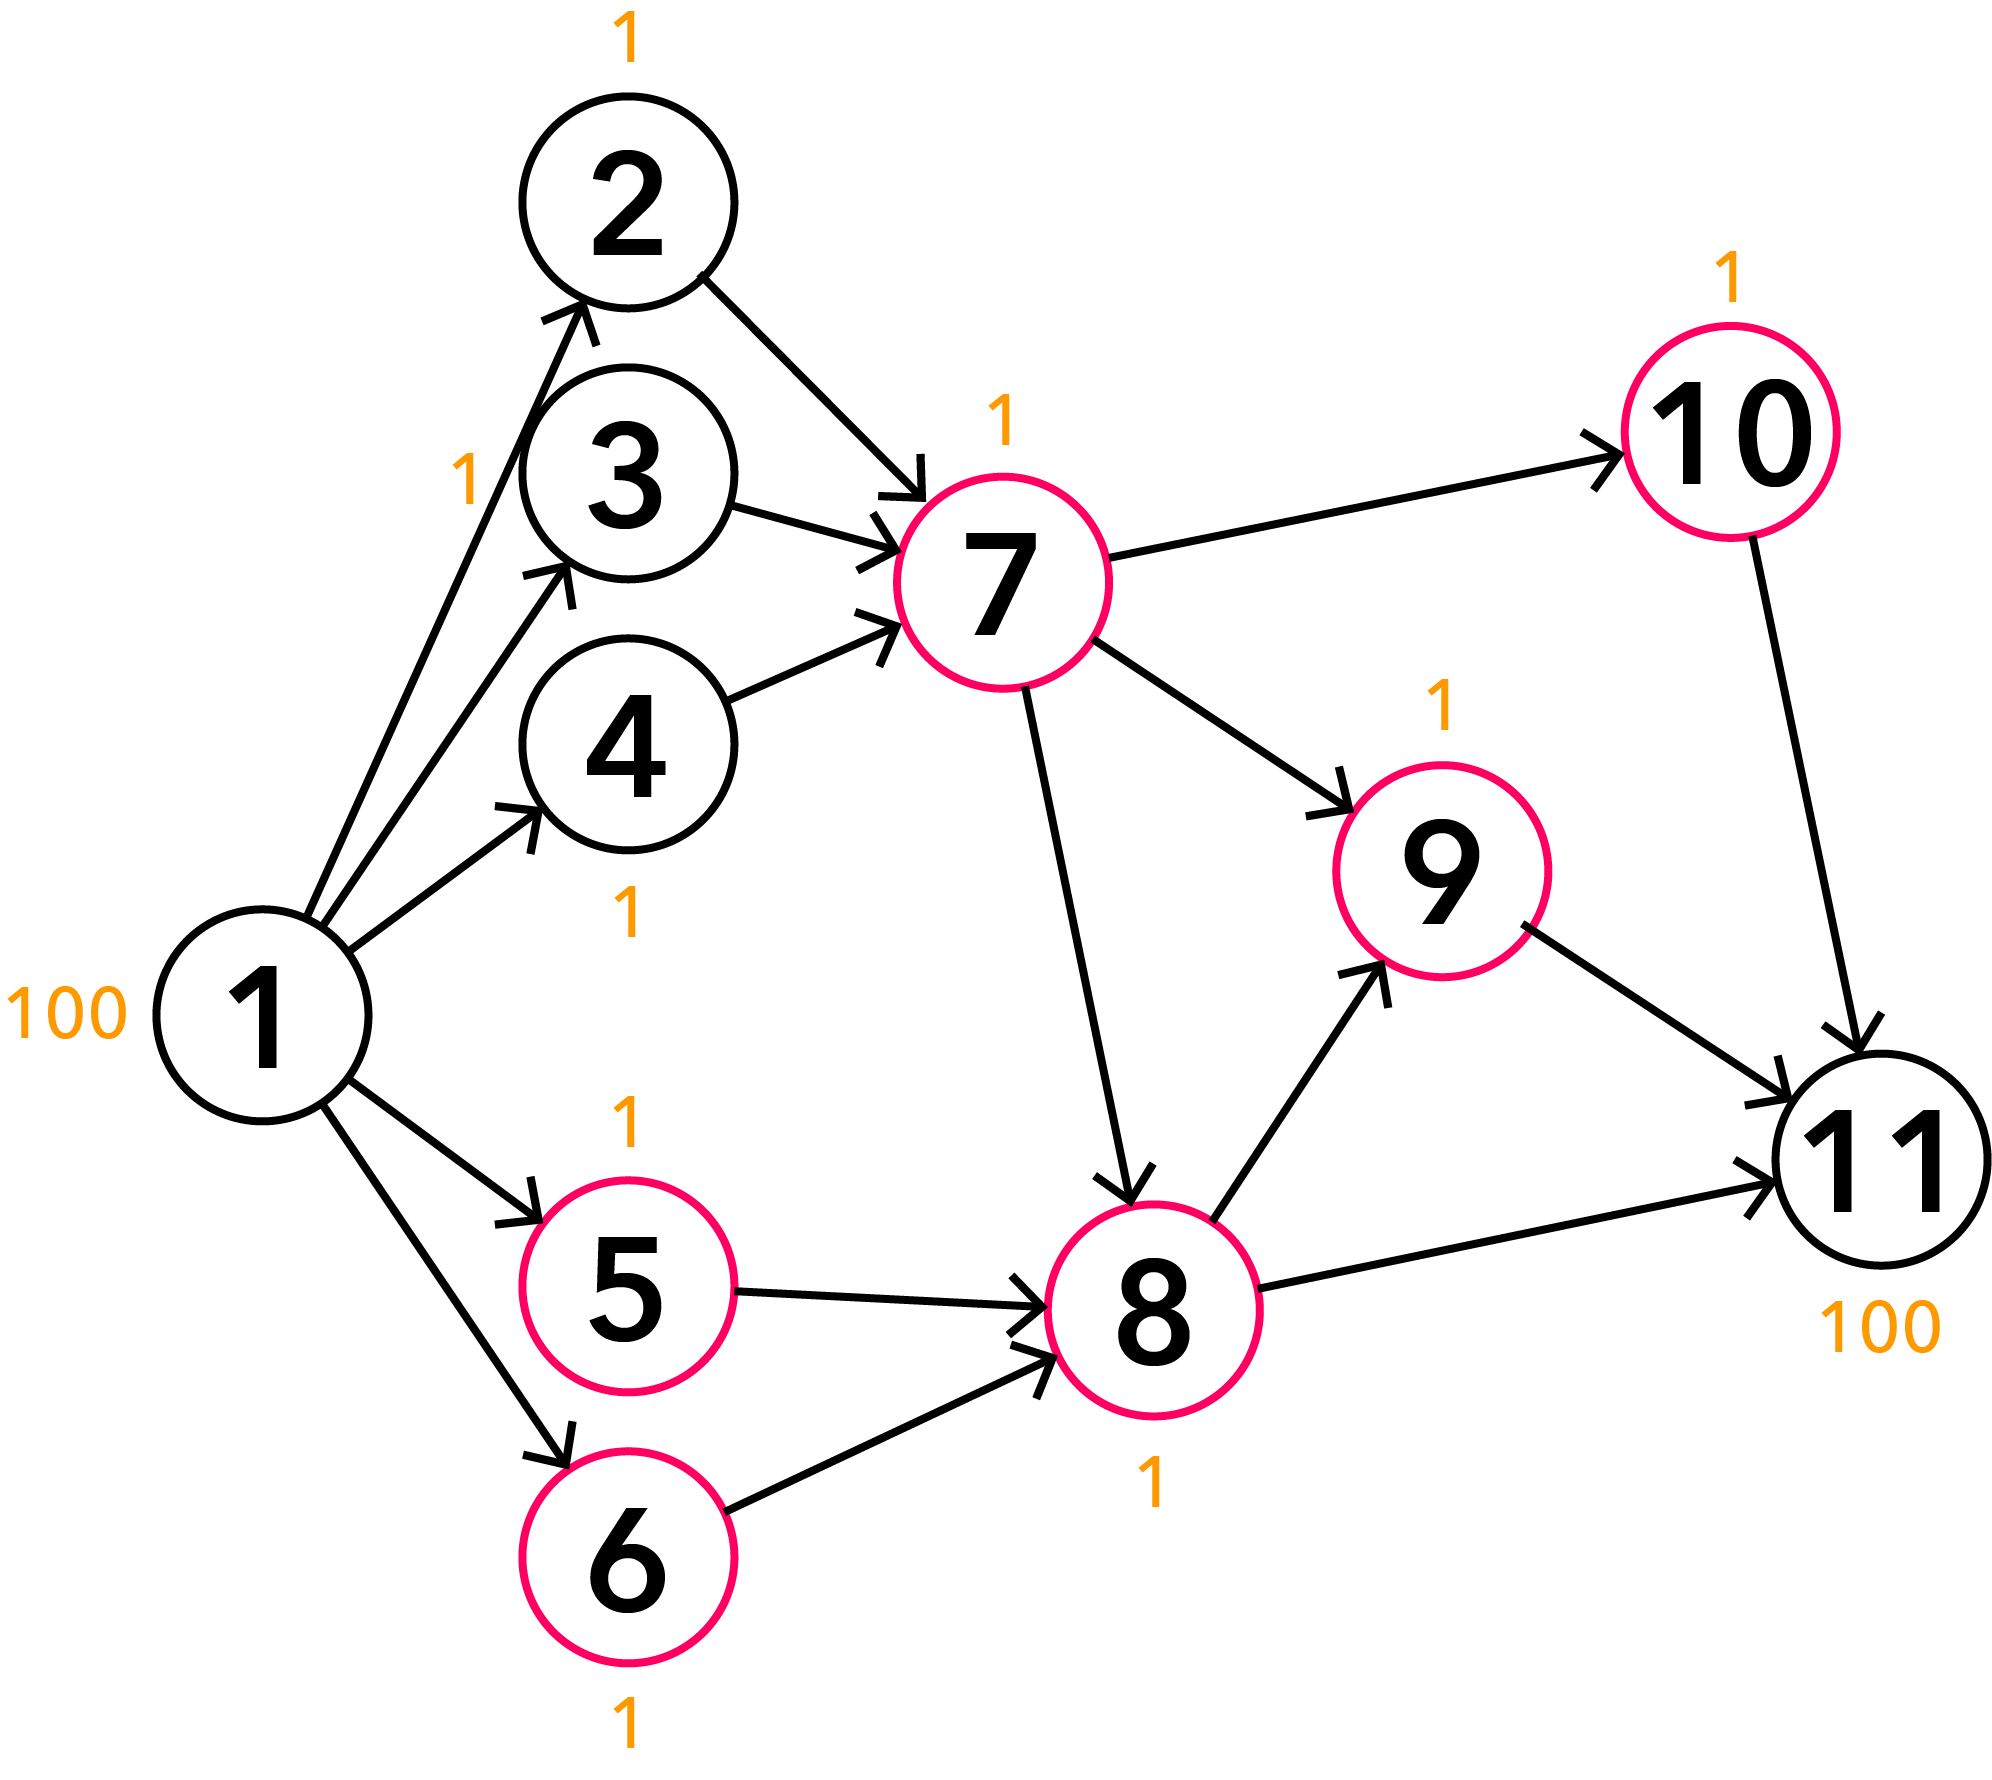
\includegraphics[width=0.30\linewidth]{../images/setting-maps/maps_sol_3.png}
    \end{center}
    
\end{frame}


\begin{frame}{\textbf{E}. 지도 설치}

    구하려는 정점 집합 $X$이 존재하지 않는 경우 (답 \texttt{-1}) 와 공집합인 경우 (답 \texttt{0}) 를 주의합시다. \newline
    supersource와 supersink를 사용하지 않은 경우 \texttt{-1}을 체크하지 못 할 수 있습니다.
    
    \vspace{0.5 \baselineskip}

    그래프의 크기는 정점이 \complexity{KN}개, 간선이 \complexity{K(N+M)}개입니다.
    
    \vspace{0.5 \baselineskip}
    
    출제자의 풀이는 \complexity{V^2 E} 시간에 동작하는 Dinic 알고리즘을 사용합니다. \newline
    이론상 최대 계산량 $K^3 N^2 M \approx 3 \times 10^8$. BOJ 기준 실행 시간 10ms, 메모리 4MiB 이내
    
    \vspace{0.5 \baselineskip}
    
    빠른 플로우 알고리즘을 사용할수록 문제는 빠르게 풀립니다. \newline
    가장 단순한 형태의 Ford-Fulkerson 알고리즘을 사용하면 시간 초과. \newline
    \complexity{VE^2}인 Edmonds-Karp 알고리즘을 사용해도 Dinic 풀이만큼 빠르게 돕니다.
    
\end{frame}